%! Author = lili
%! Date = 4/27/26

% TODO alte Folien noch einbauen
% TODO deefi Randverteilung hier?

\chapter{Unabhängigkeiten von \gls{zv}}\label{ch:unabhangigkeiten-von-zv}
\untit{Vorlesung 23 Mai 2025 (V06 2025) und Vorlesung 22.05.2026 (V05 2026)}
\begin{bsp}
    \textbf{Die Randverteilungen legen die gemeinsame Verteilung nicht eindeutig fest}  \txc{(2026)} \\
    Wir werfen eine faire Münze zweimal.
    Die Ergebnisse der beiden Würfe sollen notiert werden. \\
    Alex schreibt korrekt auf, während Kim einen Moment lang abgelenkt ist, dadurch das Ergebnis des
    zweiten Wurfs verpasst und als Notlösung einfach so tut, als hätten beide Würfe dasselbe Ergebnis
    gehabt. \\
    \textit{Modellierung}
    \[
        \eraum = \{0,1\}^2
    \]
    mit Gleichverteilung $\pe$. \\
    \textit{Zufallsvariable}
    \begin{itemize}
        \item Alex notiert den zweifachen Münzwurf \\ $\zvx : \eraum \rightarrow \eraum\ $ mit
        $\zvx = (\zvx_1, \zvx_2)$ wobei
        $\zvx_1((\ele_1, \ele_2)) = \ele_1$ und $\zvx_2((\ele_1, \ele_2)) = \ele_2$ für alle $\oio$ \\ (das heißt,
        $\zvx$ ist die Identität auf $\eraum$)
        \item Kim notiert nur den ersten Münzwurf \\ $\zvy : \eraum \rightarrow \eraum\ $ mit $\zvy = (\zvy_1, \zvy_2)$ wobei
        $\zvy_1((\ele_1, \ele_2)) = \ele_1$ und $\zvy_2((\ele_1, \ele_2)) = \zvy_1((\ele_1, \ele_2)) = \ele_1$ für alle $\oio$
    \end{itemize}
    \begin{table}[H]
        \begin{tabular}{cccc}
            $\wfk_X ((x_1, x_2))$ & $x_2 = 0$     & $x_2 = 1$     & $\wfk_{\zvx_1}(x_1)$ \\
            $x_1 = 0$             & $\frac{1}{4}$ & $\frac{1}{4}$ & $\frac{1}{2}$     \\
            $x_1 = 1$             & $\frac{1}{4}$ & $\frac{1}{4}$ & $\frac{1}{2}$     \\
            $\wfk_{\zvx_2}(x_2)$     & $\frac{1}{2}$ & $\frac{1}{2}$ & 1
        \end{tabular}

        \begin{tabular}{cccc}
            $\wfk_Y ((y_1, y_2))$ & $y_2 = 0$     & $y_2 = 1$     & $\wfk_{\zvy_1}(y_1)$ \\
            $y_1 = 0$             & $\frac{1}{2}$ & 0             & $\frac{1}{2}$     \\
            $y_1 = 1$             & 0             & $\frac{1}{2}$ & $\frac{1}{2}$     \\
            $\wfk_{\zvy_2}(y_2)$     & $\frac{1}{2}$ & $\frac{1}{2}$ & 1
        \end{tabular}\label{tab:table}
    \end{table}
    Offensichtlich sind die Randverteilungen von $\zvx$ und von $\zvy$ gleich, während die gemeinsame Verteilung
    von $\zvy_1$ und $\zvy_2$ ist nicht dieselbe ist wie jene von $\zvx_1$ und $\zvx_2$.
\end{bsp}

\begin{bsp}
    \textbf{n-mal würfeln mit fairem Würfel}  \txc{(2025)} \\
    $\eraum \{1,\dots,6\}^n, \quad \ele_i$ das Ereignis des i-ten Wurfs. $\pe$ gleichverteilt. \\
    $\zvx_i: \eraum \rightarrow \{1,\dots ,6 \}, \quad \zvx_i(\ele) = \ele_i \quad \forall i \in \{1,\dots ,6 \}$ \\
    z.z. $\zvx_i, \dots, \zvx_n$ unabhängig \\
    \begin{align*}
        \pe(\zvx_1=k_1, ..., \zvx_n= k_n) & \quad \text{ für } k_i \in \{1,..,6\} \\
        \pe(\{(k_1,..,K_n)\}) & = \frac{1}{6^n}\\
        \pe(\zvx_i = k_i)  & =
        \pe(\zvx_1\in \{1,..,6\}, ..., \zvx_{i-1} \in \{1,..,6\}, \zvx_i = k_i, \zvx_{i+1} \in \{1,..,6\}, ..., \zvx_n \in \{1,..,6\}) \\
        & = \pe(\{1,..,6\}^{i-1} \times ...) \\
        & = \frac{6^{n-1}}{6^n}
        & = \frac{1}{6}
    \end{align*}
    \[
        \pe(\zvx_1 = k_1, ..., \zvx_n = k_n)  = \pe(\zvx_1 = k_1) \cdot \dots \cdot \pe(\zvx_n = k_n)
    \]
    \txo{! jetzt müssen wir noch prüfen: Paare, Tripel, ...}
    Danach: $\zvx_1, \dots, \zvx_n$ bewiesenermaßen unabhängig \\
    Beispielsweise:
    $\Rightarrow \{x_1 \in \{2,4,6\}, \dots, \{x_4 \leq 4\}\}$ unabhängig \\
    % über arrow "z.B."
\end{bsp}
Frage: müssen wir die Paare und Tripel wirklich prüfen?

\karkar{bem_randverteilungen_legen_gemeinsame_nicht_fest}

%%%%%%%%%%%%%%%%%%%%%
% Unabhängigkeit ZV %
%%%%%%%%%%%%%%%%%%%%%
\begin{satz}  \txc{(2026)}
    Seien $\zvx_1, \dots, \zvx_n$ unabhängig $\Rightarrow \pe(\zvx_1 \in B_1 , \dots , \zvx_n \in B_n) =  \pe(\zvx_1 \in B_1) \cdot \dots \cdot \pe(\zvx_n \in B_n)$

    \paragraph{Beweis.} Um zu zeigen, dass \[\pe(\zvx_1 \in B_1, \zvx_3 = B_3) = \pe(\zvx_1 = B_3) \cdot \pe(\zvx_3 = B_3)\]
    gilt, wählen wir
    \[B_2 = E_2, B_4 = E_4 , \dots, B_n = E_n\]

\end{satz}
\begin{defi}
    \textbf{Unabhängigkeit von Zufallsvariablen}  \txc{(2026)} \\
    Auf einem Wahrscheinlichkeitsraum $\wraum$ seien Zufallsvariablen $\zvx_1, .., \zvx_n$ gegeben mit $\zvx_i : \eraum E_i$ für
    $i = 1, .., n$. \\
    Die Zufallsvariablen $\zvx_1, .., \zvx_n$ heißen unabhängig, wenn die Ereignisse
    \[
        \{\zvx_1 \in B\}, \dots , \{\zvx_n \in B\}
    \]
    für alle Wahlen von messbaren Mengen $B_i \subseteq E_i, i = 1, \dots, n$, unabhängig sind.
\end{defi}
Diese Definition ist zunächst einmal abschreckend.
Wir haben bereits gesehen, wie viele Bedingungen für den Nachweis der Unabhängigkeit von n Ereignissen zu prüfen sind.
Und nun sollen wir diesen Aufwand auch noch für jede Wahl von $B_i$ betreiben!
Wir werden uns daher im folgenden darum bemühen, einfacher nachzuweisende Kriterien für Unabhängigkeit herzuleiten.

Als erstes halten wir fest, dass es im diskreten Fall genügt, einelementige Mengen $B_i$ zu betrachten.

\section{Unabhängigkeit für Zufallsvariable mit abzählbarem Bildbereich}\label{sec:unabhangigkeit-fur-zufallsvariable-mit-abzahlbarem-bildbereich}
\komm{In 2025 und 2026 wurden diese Informationen verschieden formuliert. Hier befinden sich alle drei Versionen und eine zusammengeführte Version. Es handelt sich dabei um verschiedene Charackterisierungen der Unabhängigkeit (also es sind nur verschiedene Betrachtungsweisen des gleichen Umstands). Es sind danach auch noch weitere Charackterisierungen bzw. Konsequenzen zu finden.}
\begin{satz}
    \label{satz:satz-i}
    \textbf{Satz I. - Charakterisierung über Ereignisse}  \txc{(2025)} \\
    Seien $\zvx_1, \dots, \zvx_n$ \gls{zv} auf $(\glssymbol{eraum} , \pe); \zvx_i$ sei $E_i$-wertig. \\
    Dann
    \[
        \zvx_1, \dots, \zvx_n \text{ unabhängig } \Leftrightarrow \kl{\zvx_1 = x_1}, \dots, \kl{\zvx_n = x_n}  \text{ unabhängig } \forall x_i \in E_i (i=1, \dots, n)
    \]
    \paragraph{Beweis.} \texttt{Siehe Folie 2 (2025)}
\end{satz}


\begin{satz}
    \label{satz:satz-ii}
    \textbf{Satz II.  - Neuformulierung von Satz I. / Charakterisierung über Produktform} \txc{(2025)}  \index{Produktform} \\
    Haben $\zvx_1, \dots, \zvx_n$ abzählbare Werte-/Bildbereiche.
    Dann
    \[
        \zvx_1, \dots, \zvx_n  \text{ unabhängig } \Leftrightarrow \glssymbol{wfk}_{\zvx_1, \dots, \zvx_n} ((x_1, \dots, x_n)) = \prod^n_{i=1} \glssymbol{wfk}_{x_i}(x_i)
    \]
\end{satz}


\begin{theo}
    \label{theo:unabhaengigkeit-zv-abzaehlbar}
    \textbf{Unabhängigkeit für Zufallsvariable mit abzählbarem Bildbereich}  \txc{(2026)}\\
    Auf einem \gls{wraum} $\wraum$ seinen \glspl{zv} $\zvx_1, .., \zvx_n$ mit abzählbarem Bildbereich gegeben.
    Dann sind  $\zvx_1, .., \zvx_n$ genau dann unabhängig, wenn die Ereignisse
    \[
        \{\zvx_1 = x_1\}, \dots , \{\zvx_n = x_n\}
    \]
    für alle $x_i \in \zvx_i(\eraum), i = 1, .., n$ unabhängig sind.

    \paragraph{Beweis.} Siehe Skript S. 58.
\end{theo}

\komm{
    Gemeinsam haben alle drei Formulierungen:
    \begin{center}
        $\zvx_1, .., \zvx_n$ sind \glspl{zv} auf \gls{wraum} $\wraum$
    \end{center}
    Verschieden formuliert sind:
    \begin{center}
        ``haben abzählbare Werte-/Bildbereiche'' $\Leftrightarrow$ $\zvx_i$ sei $E_i$-wertig
    \end{center}
    und
    \[
        \zvx_1, \dots, \zvx_n \text{ unabhängig } \Leftrightarrow \overbrace{\underbrace{\kl{\zvx_1 = x_1}, \dots, \kl{\zvx_n = x_n}  \text{ unabhängig } \forall x_i \in E_i (i=1, \dots, n)}_{
            \glssymbol{wfk}_{\zvx_1, \dots, \zvx_n} ((x_1, \dots, x_n)) = \prod^n_{i=1} \glssymbol{wfk}_{x_i}(x_i)
        }}^{\text{wenn die Ereignisse }
        \{\zvx_1 = x_1\}, \dots , \{\zvx_n = x_n\}
        \text{ für alle } x_i \in \zvx_i(\eraum), i = 1, .., n \text{  unabhängig sind.}}
    \]
}


\begin{kor}
    \textbf{Konsequenz aus Satz \ref{satz:satz-ii}}  \txc{(2026)} \\
    Abzählbarer Bildbereich \\
    Es genügt
    \[\pe(\zvx_1 = x_1 , ..., \zvx_n = x_n) = \pe (\zvx_1 = x_1) \cdot \dots \cdot \pe(\zvx_n = x_n) \forall x_i \in \zvx_i(\eraum)\]
    zu zeigen, um Unabhängigkeit
    von $\zvx_1, \dots \zvx_n $ zu zeigen.
\end{kor}

% todo satz von tafel, insgesamt alles von der Tafel

\begin{satz}
    \label{satz:charaktersierung-verteilungsfunktion}
    \textbf{Charakterisierung über die Produktform der \gls{verteilungsfunktion_zv}} \txc{(2026)} \\
    $\zvx_1, .., \zvx_n$ unabhängig
    \begin{align*}
        \Leftrightarrow \pe ( \zvx_1 \leq a_1 , ..., \zvx_n \leq a_n ) & = \pe(\zvx_1 \leq a_1) \cdot \dots \cdot
        \pe(\zvx_n \leq a_n) \\
        & =  F_{\zvx_1}(a_1) \cdot \dots \cdot F_{\zvx_n}(a_n \quad \forall a_i \in \rz)
    \end{align*}
    % Fehler? vermischung von F und \pe
\end{satz}

\begin{kor}
    \label{kor:unabh-gem-verteilung-eindeutig}
    \textbf{Konsequenz aus Satz \ref{satz:charaktersierung-verteilungsfunktion}}  \txc{(2025)}\\
    $\zvx_1, .., \zvx_n$ unabhängig $\Leftrightarrow$ gemeinsame \gls{verteilung} eindeutig bestimmt durch (Rand-)\gls{verteilung}en von
    $\zvx_1, .., \zvx_n$ \\
    Aka.:
    \[
        \zvx_1, \dots, \zvx_n  \text{ unabhängig } \Rightarrow \text{ gemeinsame \gls{verteilung} von } \zvx_1, \dots, \zvx_n \text{ eindeutig bestimmt durch die Randverteilung}
    \]
\end{kor}

\begin{bem}
    Zu Korollar \autoref{kor:unabh-gem-verteilung-eindeutig}  \txc{(2025)} \\
    Das Korollar sagt uns, wie wir unabhängige Zufallsvariablen mit Zähldichte modellieren. \\
    Ohne Unabhängigkeit ist das nicht der Fall!
\end{bem}

\begin{bem}
    \textbf{Erinnerung an mathematisches Kriterium für Unabhängigkeit}  \txc{(2026)} \\
    Wie haben gesehen, dass Unabhängigkeit bereits gezeigt ist, wenn
    $\pe(\zvx_1 = x_1, \dots, \zvx_n = x_n) = \pe(\zvx_1 = x_1) \cdot .. \cdot \pe(\zvx_n = x_n) \forall x_i \in E_i (i = 1, \dots, n)$ gilt.
    \txc{Wenn also die Produktform existiert.}
    (Es ist nicht erforderlich $\zvx_{i_1}, \dots, \zvx_{i_k}$ separat zu betrachten.)
\end{bem}

\begin{bem}
    \textbf{Anwendung des mathematischen Kriteriums für Unabhängigkeit}  \txc{(2025)} \\
    \textbf{(a)} Wenn wir die Produktform finden: Beweis der Unabhängigkeit
    \txc{Wenn man also zeigen kann $\pe_{\zvx_1, \dots, \zvx_n} = \prod_i \pe_{\zvx_i}$ } \\
    \txc{Umkehridee:} \\
    \textbf{(b)} Gegeben
    \gls{verteilung} der $\zvx_i$: Wir nutzen die Produktform, um die gemeinsame \gls{verteilung} für unabhängig $\zvx_i$
    zu bestimmen.\index{Produktform}
    \txc{Also wenn die $\zvx_i$ unabhängig sind und die Randverteilungen bekannt sind, dann kann man die gemeinsame \gls{verteilung} berechnen durch
        \[
            \pe_{\zvx_1, \dots, \zvx_n} (x_1, .., x_n) = \prod_i \pe_{\zvx_i}(x_i)
        \]
    }
\end{bem}
% Tafel:
%$\zvx_1, .., \zvx_n$ mit Dichten, Unabhängigkeit
%dann
%\[
%    \pe(\zvx_1 \in a_1, \zvx_n \in a_n) = siehe bild (aber das zweite)
%\]

\karkar{def_unabhaengigkeit_zufallsvariablen_allgemein}
\karkar{satz_charakterisierung_ueber_ereignisse}
\karkar{satz_charakterisierung_ueber_produktform_abzaehlbar}
\karkar{kor_hinreichende_bedingung_unabhaengigkeit_abzaehlbar}
\karkar{satz_charakterisierung_ueber_verteilungsfunktion}
\karkar{kor_gemeinsame_verteilung_eindeutig_durch_randverteilung}
\karkar{bem_kein_separates_pruefen_von_teilmengen_noetig}
\karkar{bem_zwei_anwendungen_produktform_kriterium}


%%%%%%%%%%%%%%%%%%%%%
% Poisson-Verteilte ZV %
%%%%%%%%%%%%%%%%%%%%%

\subsection{Poisson-Verteilte ZV}\label{subsec:poisson-verteilte-zv}

%\begin{bsp}
%    \gls{verteilung} der Summe von zwei unabhängigen, Poisson-verteilten \zv \\
%    Seien $\zvx_1, \zvx_2$ unabhängig.
%    \[
%        \mu_{x_1} (k) = \pe(\zvx_1 = k) = \frac{\lambda^k_1}{k!} e^{-\lambda_1} \quad \forall k \in \nz_0
%    \]
%    \[
%        \mu_{x_2} (k) = \pe(\zvx_2 = k) = \frac{\lambda^k_2}{k!} e^{-\lambda_2} \quad \forall k \in \nz_0
%    \]
%\end{bsp}

\begin{satz}
    \textbf{Summe unabhängiger Poisson-verteilter \gls{zv} ist wieder Poisson-verteilt.}  \txc{(2025)}
    \\
    Seien $\zvx_1, \zvx_2$ unabhängig und Poisson-verteilt mit
    \begin{align*}
        \glssymbol{wfk}_{x_1}(k) = \pe(\zvx_1 = k) & = \frac{z_1^k}{k!} e^{-z_1} & (z_1 > 0) \forall k \in \mathbb{N}_0 \\
        \glssymbol{wfk}_{x_2}(k) = \pe(\zvx_2 = k) & = \frac{z_2^k}{k!} e^{-z_2} & (z_2 > 0) \forall k \in \mathbb{N}_0
    \end{align*}
    Dann gilt: $\zvx_1 + \zvx_2$ ist Poisson-Verteilt mit Parameter $z_1 + z_2$.
    \komm{$\zvx_1 + \zvx_2$ nehmen beide wete aus $\nz_0$ an, also ist die Summe auch in $\nz_0$.}

    \paragraph{Beweis.} \texttt{Siehe auch Folie 6--7 2025} \\
    $\zvx_1 + \zvx_2$ ist poisson verteilt mit Parameter $z_1 + z_2 $
    \begin{align*}
        \mu_{\zvx_1 + \zvx_2}(n) & = \pe(\zvx_1 + \zvx_2 = n) \quad \text{ für } n \in \nz_0 \\
        & = \pe \big( \uplus^k_{k_1 = 0} \{ \zvx_1 = k_1 , \zvx_2 = n - k_1\} \big) \\
        & = \sum^n_{k_1=0} \pe(\zvx_1 = k_1, \zvx_2 = n - k_1) \\
        & = \sum^n_{k_1=0} \pe(\zvx_1 = k_1) \pe(\zvx_2 = n - k_1) & \text{da unabhängig} \\
        & = \sum^n_{k_1=0} \frac{z_1^{k_1}}{k_1 !} e^{-z_1} \frac{z_2^{n-k_1}}{(n-k_1)!} e^{-z_2} \\
        & = \sum^n_{k=0} \frac{n!}{k! (n-k)!} z_1^k z_2^{n-k} & \text{durch herausziehen von }
        \big[ \frac{1}{n!} e^{-(z_1 + z_2)} \big] \\
        & = \frac{(z_1 + z_2)^n}{n!} e^{-(z_1 + z_2)}
    \end{align*}
\end{satz}

\karkar{satz_summe_unabhaengiger_poisson_verteilter_zv}

%%%%%%%%%%%%%%%%%%%%%
% Dichten ZV %
%%%%%%%%%%%%%%%%%%%%%

\section{\gls{zv} mit Dichten}\label{sec:zv-mit-dichten}

\begin{satz}
    \textbf{Satz III.: Unabhängigkeiten von \gls{zv}} (mit und ohne Dichte)  \txc{(2025)} \\
    Seien $\zvx_1, \dots, \zvx_n$ unabhängig $ \Leftrightarrow \pe(\zvx_1 \leq a_1, \dots, \zvx_n \leq a_n) = \pe(\zvx_1 \leq a_1) \cdot \dots \cdot  \pe(\zvx_n \leq a_n) = \mathcal{F}_{x_1}(a_1) \cdot \dots \cdot \mathcal{F}_{x_n}(a_n) \forall a_1, \dots, a_n \in \mathbb{R}$.

    \paragraph{Beweis.}
    \texttt{Siehe Folie 8}
\end{satz}


\begin{satz}
    \label{satz:satz-iv}
    \textbf{Satz IV.}   \txc{(2025, ergänzt 2026)}\\
    $\zvx_1, \dots, \zvx_n$ mit Dichten \index{Dichte} $f_1, \dots, f_n$.
    Dann gilt:
    $\zvx_1, \dots, \zvx_n$ unabhängig $\Leftrightarrow$ gemeinsame \dichte hat Produktform $\Leftrightarrow$ $(x_1, \dots, x_n) \mapsto f((x_1, \dots, x_n)) \coloneqq  f_1(x_1)\cdot \dots \cdot f_n(x_n)$ eine gemeinsame Sichte von $\zvx_1, \dots, \zvx_n$ ist.
\end{satz}

\begin{bem}
    Zu Satz \autoref{satz:satz-iv} \txc{(2026)} \\
    \begin{itemize}
        \item Existenz der gem. \dichte ist nicht vorausgesetzt.
        Gegeben $\zvx_1, \dots, \zvx_n$ mit Dichten \index{Dichte} $f_1, \dots, f_n$
        \item Setze
        \begin{equation}
            \label{eq:gemdichte}
            f(x_1, \dots, x_n) \coloneqq  f_1(x_1) \cdot \dots \cdot f_n(x_n) = \prod^n_{i=1} f_i(x_1) \quad \forall
            x_i \in
            \mathbb{R} (i=1, \dots, n)
        \end{equation}
        Aussage des Satzes ist: $\zvx_1, \dots, \zvx_n$ unabhängig $\Leftrightarrow f$ gem. \dichte von $\zvx_1, \dots, \zvx_n$ ist
        \item $\zvx_1, \dots, \zvx_n$ mit Dichten \index{Dichte} $f_1, \dots, f_n$.
        Modelliere unabhängige Experimente durch gemeinsame \dichte \eqref{eq:gemdichte}.
        \item Gegen eine gem. \dichte $f$ für $\zvx_1, \dots, \zvx_n$ berechne Randdichten $f_{x_1}, \dots, f_{x_n}$. \\
        Gilt Gleichung~\eqref{eq:gemdichte}? Falls ja: $\zvx_1, \dots, \zvx_n$ unabhängig.
        Falls~\eqref{eq:gemdichte} für $(x_1, \dots, x_n)$ aus einer Menge $; \subseteq \mathbb{R}^n$ gilt mit $\mathbb{R}^n\backslash M$ abzählbar, dann gilt Unabhängigkeit
    \end{itemize}
\end{bem}

\komm{Vorsicht: Eine Wahrscheinlichkeitsdichte ist nur ``fast überall'' eindeutig. \\ Also: Die Produktform muss nicht an jedem einzelnen Punkt gelten.
Es genügt, wenn sie fast überall gilt.}

%\begin{satz} \textbf{für ZV mit Dichte (2026)}\\
%$\zvx_1, .., \zvx_n$ ZV mit Dichten $f_1, .., f_n$.
%Dann gilt
%    \[
%        \zvx_1, .., \zvx_n \Rightarrow \txo{"gemDichte hat produktform"} \Rightarrow  BOLD
%    \]
%\end{satz}

\karkar{satz_unabhaengigkeit_zv_mit_dichten}
\karkar{bem_existenz_gemeinsame_dichte_nicht_vorausgesetzt}

%%%%%%%%%%%%%%%%%%%%%
% Widerlegen %
%%%%%%%%%%%%%%%%%%%%%

\section{Widerlegen von Unabhängigkeiten}\label{sec:widerlegen-von-unabhangigkeiten}
\begin{bem}
    \label{bem:widerlegen}
    Es genügt nicht einen Punkt zu finden, in dem~\eqref{eq:gemdichte} nicht gilt. \txc{(2025)} \\
    Wir brauchen eine Menge $D \subseteq \mathbb{R}^n$ mit $|D| = Z(D) > 0$, so dass~\eqref{eq:gemdichte} auf $D$ nicht gilt. \\
    Einfacher: Zeigen, dass $\pe(\zvx_1 \leq a_1, \dots, \zvx_n \leq a_n) \neq \prod^n_{i=1} F_{x_i} (a_i)$. \\
    Zeigen Sie, dass die Produktform \textbf{nicht} gilt auf Quader oder verwenden Sie die (nicht geltende) Produktform der \gls{verteilungsfunktion_zv}.
\end{bem}
\komm{
    Zu Bemerkung \autoref{bem:widerlegen}: \\
    $\pe(\zvx_1 \leq a_1, \dots, \zvx_n \leq a_n) \neq \prod^n_{i=1} F_{x_i} (a_i)$ bedeutet, die gemeinsame \gls{verteilungsfunktion_zv} faktorisiert nicht. Das ist gemeint mit ``verwenden Sie die (nicht geltende) Produktform der \gls{verteilungsfunktion_zv}'', denn da
    $F_{\zvx_1, \dots, \zvx_n}(a_1, \dots, a_n) = \pe(\zvx_1 \leq a_1, \dots, \zvx_n \leq a_n)$ gilt, ist das die Negation der Produktform der \gls{verteilungsfunktion_zv}.
}
\komm{
    Zu Bemerkung \autoref{bem:widerlegen}: \\
    Die Produktform der \gls{verteilungsfunktion_zv} wird auf sogenannten
    ``Quadern'' geprüft. Damit sind Mengen der Form
    \[
        (-\infty, a_1]\times\cdots\times(-\infty, a_n]
        \subseteq \mathbb{R}^n
    \]
    gemeint. \\
    Für den Zufallsvektor $(\zvx_1,\dots, \zvx_n)$ entspricht ein solcher Quader dem Ereignis
    \[
        \{\zvx_1\le a_1,\dots, \zvx_n\le a_n\}.
    \]
    Die gemeinsame \gls{verteilungsfunktion_zv} ist daher gerade
    \[
        F_{\zvx_1,\dots, \zvx_n}(a_1,\dots, a_n)
        =
         \pe(\zvx_1\le a_1,\dots, \zvx_n\le a_n).
    \]
    Sind $\zvx_1,\dots, \zvx_n$ unabhängig, so zerfällt diese Wahrscheinlichkeit in ein Produkt:
    \[
         \pe(\zvx_1\le a_1,\dots, \zvx_n\le a_n)
        =
        \prod_{i=1}^n  \pe(\zvx_i\le a_i)
        =
        \prod_{i=1}^n F_{\zvx_i}(a_i).
    \]
    Man sagt dann: \\
    Die \gls{verteilungsfunktion_zv} besitzt Produktform auf Quadern. \\
    Um zu zeigen, dass Zufallsvariablen nicht unabhängig sind, genügt es daher,
    einen Quader zu finden, für den diese Produktform nicht gilt. \index{Produktform} \\
    \chatti
}
% todo 2025  Randdichten: BSP  \texttt{Hier fehlt was}


\komm{Bei Bild Tafel link ganz unten reicht es an einem Punkt zu zeigen, weil wir da ganze Mengen benutzt haben. Heh?}

\begin{bsp}
    \textbf{uniform. verteilung auf Rechteck} \txc{(2026)} \\
    Sei $(\zvx, \zvy)$ ein zufälliger Punkt in $\rz$ (uniforme Verteilung)
    \begin{figure}[H]
        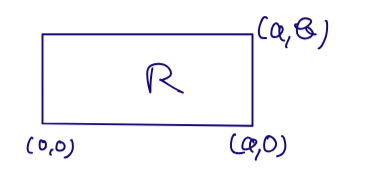
\includegraphics[width=0.4\linewidth]{./images/viereck}\label{fig:figure2}
    \end{figure}
    $(\zvx, \zvy)$ hat (gem.) Dichte $f(x, y) = \chaf_R (x, y) \frac{1}{a \cdot b} \quad \forall (x, y) \in \rz^2$
    Randdichten:
    \begin{align*}
        f_X(x) = \chaf_{[0, a]}(x) \in_0^b \underbrace{f(x, y)}_{\frac{1}{a \cdot b}} dy & = \frac{1}{a} \chaf_{[0, a]}(x)\\
        f_Y(y) & = \frac{1}{b} \chaf_{[0, b]}(y)\\
        f(x, y)&  = \chaf_{[0, a] \times [0, b]}(x, y)  \frac{1}{a \cot b} \\
        & = f_X(x) f_Y(y)
    \end{align*}
    schlauer:
    \[
        f(x, y) = \chaf_{\rz} (x, y) \frac{1}{a \cot b} = \frac{1}{a} \underbrace{\chaf_{[0, a]}(x) }_{\text{Randdichte von } \zvx} \cdot \frac{1}{b} \underbrace{\chaf_{[0, b]}(y) }_{\text{Randdichte von } \zvy}
    \]
    \txo{Wir müssen die Randdichten gar nicht berechnen!}
    $\zvx, \zvy$ unabhängig
    \komm{wenn man sieht die Dichte zerfällt in x und y Argument muss man nicht integrieren, sondern nur schauen, dass die Funktionen (?) das richtige Gewicht haben. OK. Gerald fragen...} % TODO
\end{bsp}

\begin{bsp}
    \label{bsp:dreieck}
    Dreieck \txc{(2026)}
    \begin{figure}[H]
        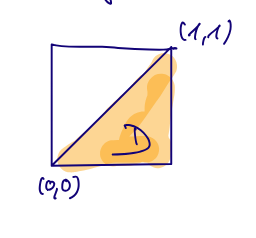
\includegraphics[width=0.3\linewidth]{./images/dreieck}\caption{}\label{fig:dreieck}
    \end{figure}
    Sei $(\zvx, \zvy)$ ein zufälliger Punkt \txc{gleichverteilt} im Dreieck $D$. \\
    \txc{Gleichverteilt bedeutet: Dichte ist konstant auf $D$ und 0 außerhalb.}
    \begin{align*}
        f(x, y) & = \frac{1}{|D|} \chaf_D (x, y) \\
        & = 2 \chaf_D(x, y) \\
        & = \begin{cases}
                2 & 0 \leq y \leq x \leq 1 \\ 0 & sonst
        \end{cases}
    \end{align*}
    Randdichten: \txc{(Man ``integriert die andere Variable weg'')})
    \begin{align*}
        f_X (x) & = \chaf_{[0,1]}(x) \int_{- \infty}^{\infty} f(x, y) dy \\
        & = \chaf_{[0,1]}(x) \int_{0}^{\txo{x}} 2 dy = 2 x  \chaf_{[0,1]}(x) \\
        f_Y (y) & = \dots = 2(1-y)\chaf_{[0,1]}(y)
    \end{align*}
    Wenn $\zvx, \zvy$ unabhängig \txc{wären, dann würde gelten}:
    \txc{\begin{equation}
             f(x, y) = f_X(x)\, f_Y(y)\label{eq:wenn-unabhaengig}
    \end{equation}}
    \txc{Einsetzen ergibt:}
    \begin{align*}
        f(x, y) & = 2 \cdot \chaf_D(x, y) \\
        & \overset{?}{=} f_X(x) f_Y(y) \\
        & = 2x 2 (1-y) \chaf_{[0,1]}(x, y)
    \end{align*}
    Wir sehen:
    Für $(x, y) \in [0,1]^2 \backslash D $ gilt $f(x, y) = 0$, also
    ``rechte Seite'' $> 0$. \\
    Keine Unabhängigkeit. \txc{Für Erklärung siehe Kommentar \ref{kom:dreieck-erklaert}.} \\
    Alternative:
    \txc{Statt Dichten zu vergleichen, kann man Unabhängigkeit auch testen über:
        \[
             \pe(\zvx\le a, \zvy\le b) \stackrel{?}{=} \fxx(a)\fxy(b)
        \]}
    Explizit: Berechne $\fxx$ und $\fxy$, zeige, dass eis \textbf{einen} Punkt $(a, b) \in \rz^2$ gibt mit
    \[
        \pe(\zvx \leq a, \zvy \leq b) \neq \fxx(a) \fxy(b).
    \]
\end{bsp}

\komm{Symbole und Terme in Beispiel \autoref{bsp:dreieck}
    \begin{itemize}
        \item $\chaf_D(x, y)$ = Indikatorfunktion:
        \[
            \chaf_D(x, y)=
            \begin{cases}
                1 & (x, y)\in D \\
                0 & \text{sonst}
            \end{cases}
        \]
        \item $|D|$ = Fläche des Dreiecks (hier: $|D|=\tfrac12$)
        \item $f(x, y)$ = gemeinsame Dichte von $(\zvx, \zvy)$
        \item $f_X(x)$ beschreibt die \gls{verteilung} von $\zvx$ alleine
        \item $f_Y(y)$ beschreibt die \gls{verteilung} von $\zvy$ alleine
    \end{itemize}
}

\komm{ \label{kom:dreieck-erklaert}
Für $(x, y) \in [0,1]^2 \backslash D $ gilt $f(x, y) = 0$
    weil in der Dichtefunktion oben explizit festgelegt wird, dass es außerhalb des Dreiecks 0 ist und $[0,1]^2 \backslash D$ ist alles außer das Dreieck. \\ Also
    ist die ``rechte Seite''  $f_X(x)\, f_Y(y)$ aus \ref{eq:wenn-unabhaengig}). \\
    Diese ist $> 0$, denn $x$ kann 0 sein (siehe Bild \ref{fig:dreieck}, 0 ist der innerste Randpunkt von ``außerhalb des Dreiecks'') und
    $y$ kann 1 sein (analog äußerster Randpunkt von ``außerhalb des Dreiecks''). Aber da es Randpunkte sind, haben sie keinen Einfluss auf die Dichte, denn Punkte haben keine Fläche und somit keine relevante ``Menge''. Also kann man diese Punkte
    wegignorieren und einfach sagen $x > 0$ und $y < 1$. Und wenn man das annimmt, dann erhält man:
    \[
        f_X(x) f_Y(y) = 4 x (1-y) \chaf_{[0,1]^2}(x, y)
    \]
    Denn wir haben ja oben ausgerechnet, dass $f_X (x) = 2 x  \chaf_{[0,1]}(x)$ und $f_Y (y) = 2(1-y)\chaf_{[0,1]}(y)$, INSOFERN $\zvx$ und $\zvy$ unabhängig sind. \\
    Weil aber $y<1$ gilt, muss $1-y>0$ sein, also
    \[
        \overbrace{ 4  \underbrace{x}_{> 0}  ( \underbrace{1-y}_{> 0} )}^{> 0}
    \]
    Das ist dann ein Widerspruch damit, dass jeder Punkt außerhalb des Dreiecks $f(x, y) = 0$ hat. Wir haben einen Punkt außerhalb des Dreiecks betrachtet, und der hatte
    $f_X(x) f_Y(y) > 0$. Also $ f(x, y) \neq f_X(x) f_Y(y)$, was äauivalet ist zu ``$\zvx$ und
    $\zvy$ sind NICHT unabhängig''.
}

\komm{Zu Beispiel \autoref{bsp:dreieck} \\
\textbf{Warum reicht ein einzelner Punkt zur Widerlegung?}
Wenn Unabhängigkeit gilt, muss die Gleichung für \emph{alle} $(a, b)$ gelten. Findet man \emph{einen einzigen} Punkt $(a, b)$ mit Ungleichheit,
    ist Unabhängigkeit widerlegt. \\
    "Unabhängigkeit ist eine globale Eigenschaft und ein Gegenbeispiel genügt, um sie zu zerstören."
}

\karkar{bem_widerlegen_von_unabhaengigkeit_dichte}
\karkar{def_quader_und_produktform_darauf}
\karkar{bem_produktform_direkt_ablesbar_ohne_randdichten}
\karkar{bem_gebietsgrenze_typische_ursache_fuer_abhaengigkeit}
\karkar{bem_unabhaengigkeit_globale_eigenschaft}

%%%%%%%%%%%%%%%%%%%%%
% Faltung %
%%%%%%%%%%%%%%%%%%%%%

\begin{defi} \textbf{Faltung} \txc{(2026)} \\
    $\zvx, \zvy$ unabhängig \zv.
    Dann heißt die \gls{verteilung} der Summe \textbf{Faltung} (der \gls{verteilung}en). \index{Faltung}
\end{defi}

\karkar{def_faltung}




